% Flamingo gated cross-attention — TikZ source. Compiles to a tight standalone
% PDF (pdflatex figures/gated-xattn.tex), which `book-scaffold build-figures`
% converts to public/figures/gated-xattn.svg (PDF -> SVG via pdftocairo).
%
% The cross-attention output is scaled by tanh(gamma) before the residual add.
% At gamma=0 the gate is closed and f_aug = f_LM; gradient reaches gamma first.
\documentclass[tikz,border=3pt]{standalone}
\usepackage{amsmath}
\usepackage{amssymb}
\usepackage{tikz}
\usetikzlibrary{positioning,arrows.meta,calc}
\begin{document}
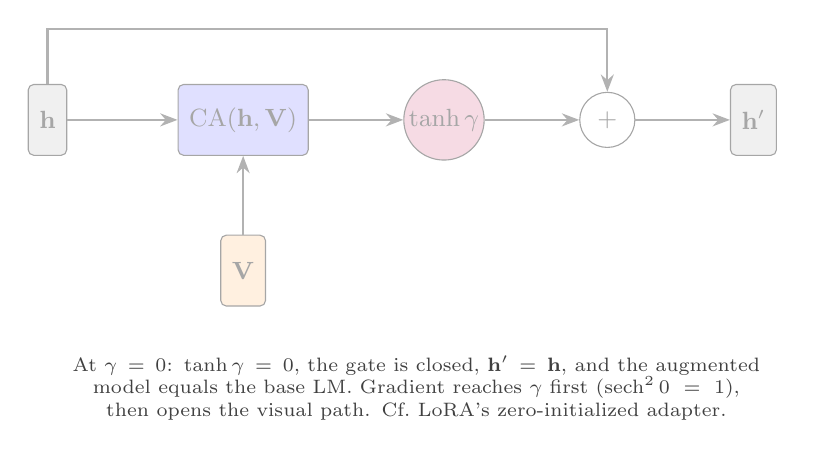
\begin{tikzpicture}[
    font=\small,
    box/.style={draw, gray!70, rounded corners=2pt, align=center,
                minimum height=9mm, inner sep=4pt},
    gate/.style={draw, gray!70, circle, inner sep=1pt, minimum size=8mm,
                 fill=purple!14},
    add/.style={draw, gray!70, circle, inner sep=1pt, minimum size=7mm},
    op/.style={->, >={Stealth[length=2.2mm]}, gray!60, thick},
  ]
  % residual stream in
  \node[box, fill=black!6] (hin) {$\mathbf h$};
  % cross-attention
  \node[box, fill=blue!12, right=14mm of hin] (ca) {$\operatorname{CA}(\mathbf h,\mathbf V)$};
  % gate
  \node[gate, right=12mm of ca] (g) {$\tanh\gamma$};
  % add
  \node[add, right=12mm of g] (plus) {$+$};
  % out
  \node[box, fill=black!6, right=12mm of plus] (hout) {$\mathbf h'$};

  % visual features feeding CA
  \node[box, fill=orange!12, below=10mm of ca] (V) {$\mathbf V$};

  \draw[op] (hin) -- (ca);
  \draw[op] (ca) -- (g);
  \draw[op] (g) -- (plus);
  \draw[op] (plus) -- (hout);
  \draw[op] (V) -- (ca);

  % residual skip
  \draw[op] (hin.north) |- ($(hin.north)+(0,7mm)$) -| (plus.north);

  \node[below, align=center, text width=9.5cm, font=\scriptsize, text=black!75]
    at ($(V.south)+(2.2,-0.5)$)
    {At $\gamma=0$: $\tanh\gamma=0$, the gate is closed, $\mathbf h'=\mathbf h$, and the
     augmented model equals the base LM. Gradient reaches $\gamma$ first
     ($\operatorname{sech}^2 0=1$), then opens the visual path. Cf.\ LoRA's
     zero-initialized adapter.};
\end{tikzpicture}
\end{document}
